%% ===========================================================================
%%  Exoplanet Transit Detection -- 4-Week Winter Project Guide
%%  Astronomy Club Winter Project
%%
%%  Build:   pdflatex exoplanet_project_guide
%%           bibtex   exoplanet_project_guide
%%           pdflatex exoplanet_project_guide   (x2)
%%  or just: latexmk -pdf exoplanet_project_guide.tex
%%
%%  Uses only packages found in a *basic* TeX Live install (plus Overleaf),
%%  so it compiles anywhere.
%% ===========================================================================
\documentclass[11pt,a4paper]{article}

% ---------------------------------------------------------------- packages --
\usepackage[T1]{fontenc}
\usepackage[utf8]{inputenc}
\usepackage{amsmath,amssymb}
% Fonts: Palatino-style (newpx) + TeX Gyre Heros headings when installed
% (Overleaf, full TeX Live); otherwise fall back to Latin Modern.
\IfFileExists{newpxtext.sty}{%
  \usepackage{newpxtext,newpxmath}%
  \IfFileExists{tgheros.sty}{\usepackage[scale=0.9]{tgheros}}{}%
}{%
  \usepackage{lmodern}%
}
\renewcommand{\ttdefault}{lmtt}             % Latin Modern mono everywhere
\usepackage[margin=2.3cm,top=2.6cm,bottom=2.6cm,headheight=14pt]{geometry}
\usepackage[dvipsnames,table]{xcolor}
\usepackage{graphicx}
\usepackage{tikz}
\usetikzlibrary{calc,positioning,shapes.geometric,arrows.meta,decorations.pathreplacing}
\usepackage{booktabs,tabularx,longtable,array,colortbl,multicol}
\usepackage{fancyhdr}
\usepackage{pifont}
\usepackage{caption}
\usepackage{float}
\usepackage{verbatim}                      % lets \verbatim live inside a custom environment
\usepackage[numbers,sort&compress]{natbib}
\usepackage{url}
\usepackage[colorlinks=true,linkcolor=navy,urlcolor=teal,citecolor=teal,
            bookmarksnumbered=true,pdftitle={Exoplanet Transit Detection: 4-Week Winter Project Guide},
            pdfauthor={Astronomy Club}]{hyperref}
\usepackage{bookmark}

% ------------------------------------------------------------------ colours --
\definecolor{navy}{HTML}{1B2A4A}
\definecolor{night}{HTML}{0E1626}
\definecolor{amber}{HTML}{E8A33D}
\definecolor{teal}{HTML}{1F7A70}
\definecolor{brick}{HTML}{C0503A}
\definecolor{plum}{HTML}{6A4C93}
\definecolor{leaf}{HTML}{3F8F3F}
\definecolor{softgrey}{HTML}{F3F4F6}
\definecolor{codeline}{HTML}{B8C0CC}

% ----------------------------------------------------------- page styling --
\setlength{\parindent}{0pt}
\setlength{\parskip}{0.55em}
\linespread{1.06}
\pagestyle{fancy}
\fancyhf{}
\renewcommand{\headrulewidth}{0.4pt}
\renewcommand{\headrule}{{\color{codeline}\hrule width\headwidth height\headrulewidth}}
\fancyhead[L]{\sffamily\footnotesize\color{navy}Exoplanet Transit Detection \textperiodcentered{} Winter Project}
\fancyhead[R]{\sffamily\footnotesize\color{navy}\leftmark}
\fancyfoot[C]{\sffamily\footnotesize\color{navy}\thepage}
\renewcommand{\sectionmark}[1]{\markboth{#1}{}}

% section headings without titlesec
\makeatletter
\renewcommand\section{\@startsection{section}{1}{\z@}%
  {-3.0ex \@plus -1ex \@minus -.2ex}{1.4ex \@plus .2ex}%
  {\normalfont\sffamily\LARGE\bfseries\color{navy}}}
\renewcommand\subsection{\@startsection{subsection}{2}{\z@}%
  {-2.6ex\@plus -1ex \@minus -.2ex}{0.8ex \@plus .2ex}%
  {\normalfont\sffamily\Large\bfseries\color{navy}}}
\renewcommand\subsubsection{\@startsection{subsubsection}{3}{\z@}%
  {-2.0ex\@plus -1ex \@minus -.2ex}{0.5ex \@plus .2ex}%
  {\normalfont\sffamily\large\bfseries\color{teal}}}
\def\@seccntformat#1{{\color{amber}\csname the#1\endcsname}\hspace{0.6em}}
\renewcommand{\verbatim@font}{\normalfont\ttfamily\small\hyphenchar\font\m@ne\@noligs}
% let long URLs break anywhere
\g@addto@macro{\UrlBreaks}{\do\/\do\a\do\b\do\c\do\d\do\e\do\f\do\g\do\h\do\i\do\j\do\k\do\l\do\m\do\n\do\o\do\p\do\q\do\r\do\s\do\t\do\u\do\v\do\w\do\x\do\y\do\z\do\-\do\_\do\.\do\=\do\?\do\&}
\makeatother
\urlstyle{tt}

% compact lists (no enumitem needed)
\let\olditemize\itemize
\renewcommand{\itemize}{\olditemize\setlength{\itemsep}{2pt}\setlength{\parskip}{0pt}\setlength{\parsep}{0pt}}
\let\oldenumerate\enumerate
\renewcommand{\enumerate}{\oldenumerate\setlength{\itemsep}{2pt}\setlength{\parskip}{0pt}\setlength{\parsep}{0pt}}
\renewcommand{\labelitemi}{{\color{amber}\small$\blacktriangleright$}}

% checklists
\newenvironment{checklist}{\begin{itemize}\renewcommand{\labelitemi}{\color{teal}\ding{113}}}{\end{itemize}}

% ---------------------------------------------------- callout boxes (tikz) --
\newsavebox{\calloutbox}
\newenvironment{callout}[3]% #1 colour, #2 symbol, #3 title
 {\def\cocolor{#1}%
  \begin{lrbox}{\calloutbox}\begin{minipage}{\dimexpr\linewidth-1.6em\relax}\small
  \setlength{\parskip}{0.4em}%
  {\sffamily\bfseries\color{#1}#2\hspace{0.45em}#3}\par}
 {\end{minipage}\end{lrbox}%
  \par\medskip\noindent
  \begin{tikzpicture}
    \node[inner sep=0.8em, fill=\cocolor!7, anchor=north west] (b) at (0,0) {\usebox{\calloutbox}};
    \draw[line width=2.6pt, \cocolor] (b.north west) -- (b.south west);
  \end{tikzpicture}\par\medskip}

\newenvironment{checkpoint}{\begin{callout}{teal}{\ding{52}}{Checkpoint}}{\end{callout}}
\newenvironment{goingfurther}{\begin{callout}{plum}{\ding{72}}{Going further (full-time / extra keen)}}{\end{callout}}
\newenvironment{pitfall}{\begin{callout}{brick}{\ding{110}}{Pitfalls we have seen}}{\end{callout}}
\newenvironment{keyidea}{\begin{callout}{amber}{\ding{228}}{Key idea}}{\end{callout}}
\newenvironment{reading}{\begin{callout}{navy}{\ding{45}}{Reading for this week}}{\end{callout}}
\newenvironment{instructor}{\begin{callout}{leaf}{\ding{80}}{Note for organisers}}{\end{callout}}

% code blocks with hairlines (verbatim can't live in a box without extra packages)
\newenvironment{code}%
 {\par\smallskip\noindent{\color{codeline}\rule{\linewidth}{0.6pt}}\par\vspace{-0.9\baselineskip}\verbatim}%
 {\endverbatim\vspace{-0.6\baselineskip}\noindent{\color{codeline}\rule{\linewidth}{0.6pt}}\par\smallskip}

% resource entry: \res{Name}{url}{why}
\newcommand{\res}[3]{\item \textbf{\href{#2}{#1}} --- #3\\[-1pt]{\scriptsize\color{gray}\url{#2}}}
\newenvironment{reslist}{\begin{itemize}\setlength{\itemsep}{5pt}}{\end{itemize}}

% week banner: \weekbanner{number}{title}{subtitle}
\newcommand{\weekbanner}[3]{%
  \par\noindent
  \begin{tikzpicture}
    \fill[navy] (0,0) rectangle (\linewidth,1.9);
    \fill[amber] (0,0) rectangle (0.22,1.9);
    \node[anchor=west,text=amber,font=\sffamily\bfseries\Huge] at (0.6,0.95) {#1};
    \node[anchor=south west,text=white,font=\sffamily\bfseries\LARGE] at (2.0,0.85) {#2};
    \node[anchor=north west,text=white!80!navy,font=\sffamily\normalsize] at (2.0,0.8) {#3};
  \end{tikzpicture}\par\medskip}

% hours pill
\newcommand{\hrs}[1]{\tikz[baseline=(h.base)]\node[fill=amber!25,rounded corners=2pt,inner sep=1.5pt,font=\sffamily\scriptsize](h){#1};}

% shorthand
\newcommand{\Rearth}{\ensuremath{R_\oplus}}
\newcommand{\Rsun}{\ensuremath{R_\odot}}
\newcommand{\Rstar}{\ensuremath{R_\star}}
\newcommand{\pkg}[1]{\texttt{#1}}
\newcolumntype{Y}{>{\raggedright\arraybackslash}X}
\newcolumntype{L}[1]{>{\raggedright\arraybackslash}p{#1}}
\renewcommand{\arraystretch}{1.25}

% =============================================================== document ==
\begin{document}

% ------------------------------------------------------------------- cover --
\begin{titlepage}
\thispagestyle{empty}
\begin{tikzpicture}[remember picture,overlay]
  \fill[night] (current page.south west) rectangle (current page.north east);
  % stars
  \pgfmathsetseed{271828}
  \foreach \i in {1,...,260}{
    \pgfmathsetmacro{\x}{rnd*21}\pgfmathsetmacro{\y}{rnd*29.7}\pgfmathsetmacro{\r}{0.008+rnd*0.03}
    \fill[white,opacity=0.35+0.5*rnd] ($(current page.south west)+(\x,\y)$) circle (\r);}
  % the star and its planet
  \shade[inner color=amber!40!white, outer color=amber!60!brick]
     ($(current page.north east)+(-5.2,-7.6)$) circle (3.4);
  \fill[night] ($(current page.north east)+(-6.4,-7.0)$) circle (0.55);
  % a light curve across the page
  \begin{scope}[shift={($(current page.south west)+(1.5,8.2)$)}]
    \draw[white!40!night,thin] (0,0) -- (18,0);
    \pgfmathsetseed{4}
    \foreach \t in {0,0.06,...,18}{
      \pgfmathsetmacro{\ph}{mod(\t+0.6,4.5)}
      \pgfmathsetmacro{\dip}{-0.6*max(0,min(1,min(\ph/0.22,(1.1-\ph)/0.22)))}
      \pgfmathsetmacro{\yy}{1.4+\dip+0.12*rand}
      \fill[amber!85!white] (\t,\yy) circle (0.035);}
    \node[anchor=north west,text=white!60!night,font=\sffamily\footnotesize] at (0,-0.15)
       {time $\longrightarrow$ \qquad (every dip is the same planet passing in front of its star)};
  \end{scope}
  % titles
  \node[anchor=north west,text=amber,font=\sffamily\bfseries\large]
     at ($(current page.north west)+(1.8,-2.2)$) {ASTRONOMY CLUB \textperiodcentered{} WINTER PROJECT};
  \node[anchor=north west,text=white,font=\sffamily\bfseries\fontsize{34}{38}\selectfont,align=left]
     at ($(current page.north west)+(1.8,-3.3)$) {Exoplanet\\Transit\\Detection};
  \node[anchor=north west,text=white!85!night,font=\sffamily\Large,align=left]
     at ($(current page.north west)+(1.8,-9.6)$)
     {Find a planet in NASA data, measure it,\\and then measure how good \emph{you}\\are at finding planets.};
  \node[anchor=north west,text=white!70!night,font=\sffamily\normalsize,align=left,text width=16cm]
     at ($(current page.north west)+(1.8,-12.4)$)
     {A four-week, ground-up project track: Kepler \& TESS light curves from MAST
      $\cdot$ detrending $\cdot$ Box Least Squares $\cdot$ transit fitting $\cdot$
      planet radii $\cdot$ injection--recovery and pipeline completeness.};
  \node[anchor=south west,text=white!60!night,font=\sffamily\small,align=left]
     at ($(current page.south west)+(1.8,2.0)$)
     {Project guide, resource compendium \& week-by-week plan\\
      Companion code: \texttt{exoplanet-transit-winter-project} (GitHub)\\
      Version 1.0 \textperiodcentered{} \today};
\end{tikzpicture}
\end{titlepage}

% ------------------------------------------------------------ at a glance --
\pagenumbering{roman}
\section*{At a glance}
\markboth{At a glance}{}
\addcontentsline{toc}{section}{At a glance}

\textbf{The project in one sentence.} Over four weeks you will write your own pipeline that downloads a
real star's brightness measurements from NASA, finds a periodic dip caused by an orbiting planet, measures
that planet's size, and then tests the pipeline on thousands of \emph{fake} planets to measure exactly which
planets it can and cannot find.

\textbf{Why the twist matters.} Finding a known planet is a tutorial. Measuring your own pipeline's
\emph{detection efficiency} is research: it is the step that turns ``we found 10 planets'' into ``planets of
this size are this common''. The Kepler team did exactly this to calibrate its final
catalogue~\citep{Christiansen2020}. By the end of Week~4 you will have done a small version of it yourself.

\begin{center}
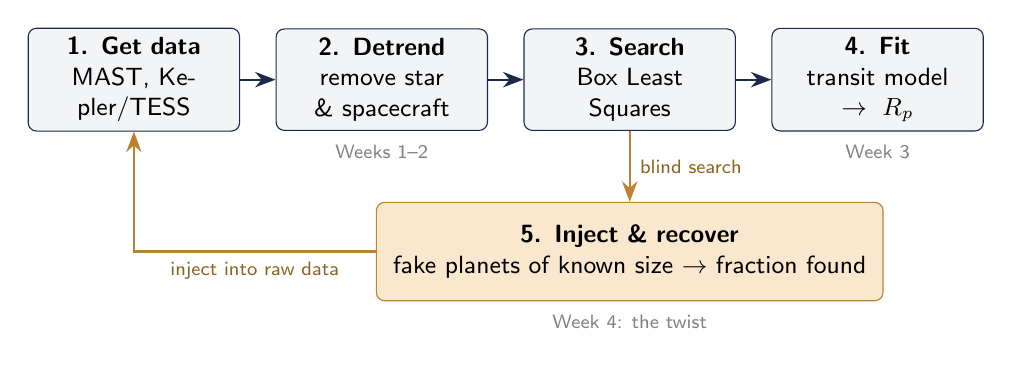
\begin{tikzpicture}[
  stage/.style={draw=navy,fill=softgrey,rounded corners=3pt,minimum height=1.25cm,text width=2.45cm,
                align=center,font=\sffamily\small},
  arr/.style={-{Stealth[length=2.6mm]},thick,navy}]
  \node[stage] (a) {\textbf{1. Get data}\\ MAST, Kepler/TESS};
  \node[stage,right=0.45cm of a] (b) {\textbf{2. Detrend}\\ remove star \& spacecraft};
  \node[stage,right=0.45cm of b] (c) {\textbf{3. Search}\\ Box Least Squares};
  \node[stage,right=0.45cm of c] (d) {\textbf{4. Fit}\\ transit model $\to R_p$};
  \node[stage,fill=amber!25,draw=amber!80!black,below=0.9cm of c,text width=6.2cm] (e)
      {\textbf{5. Inject \& recover}\\ fake planets of known size $\to$ fraction found};
  \draw[arr] (a)--(b); \draw[arr] (b)--(c); \draw[arr] (c)--(d);
  \draw[arr,amber!80!black] (e.west) -| node[pos=0.25,below,font=\sffamily\scriptsize,text=amber!60!black]{inject into raw data} (a.south);
  \draw[arr,amber!80!black] (c.south) -- node[right,font=\sffamily\scriptsize,text=amber!60!black]{blind search} (e.north);
  \node[font=\sffamily\scriptsize,text=gray,below=0.05cm of b] {Weeks 1--2};
  \node[font=\sffamily\scriptsize,text=gray,below=0.05cm of d] {Week 3};
  \node[font=\sffamily\scriptsize,text=gray,below=0.05cm of e] {Week 4: the twist};
\end{tikzpicture}
\end{center}

\vspace{-0.5em}
\begin{center}
\small
\begin{tabularx}{\linewidth}{@{}l Y l@{}}
\toprule
\textbf{Week} & \textbf{Theme and what you will have at the end} & \textbf{Notebook}\\
\midrule
1 & \textbf{Foundations.} Python crash course, GitHub, transit physics; a real Kepler light curve on screen, your own target chosen. & 00, 01\\
2 & \textbf{Find it.} Detrending + Box Least Squares; Kepler-10\,b recovered from raw NASA data; your target searched. & 02\\
3 & \textbf{Measure it.} Transit model fit, error bars, planet radius compared with the literature. & 03\\
4 & \textbf{Know your limits.} Injection--recovery completeness map, one controlled experiment, report and talk. & 04\\
\bottomrule
\end{tabularx}
\end{center}

\begin{multicols}{2}
\textbf{Time.} Core track \textbf{10--15\,h/week}: two club sessions (\(\sim\)2\,h and \(\sim\)3\,h) plus self-paced work.
Every week also has a \emph{Going further} box for students who want to (or can) work full-time.

\textbf{Who.} Freshmen to seniors. No coding experience is assumed: Week~1 starts from
\texttt{print("hello")}. Seniors are expected to go further and to help.

\textbf{Format.} Every student builds their \emph{own} GitHub repository: it is your portfolio piece.
Collaboration and help are encouraged; the code, figures and write-up in your repo must be your own.

\columnbreak
\textbf{Final deliverables (Section~\ref{sec:deliverables}).}
\begin{itemize}
  \item A public GitHub repo that runs from top to bottom.
  \item A 4--6 page paper-style report (template provided).
  \item A 5-minute talk or a poster at Demo Day.
\end{itemize}

\textbf{Software.} Python, NumPy, Matplotlib, Astropy, Lightkurve; optional batman, wotan, emcee.
Runs in Google Colab (zero install) or locally (Section~\ref{sec:setup}).
\end{multicols}

\newpage
\tableofcontents
\newpage
\pagenumbering{arabic}

% =========================================================================
\section{Why this project?}
\label{sec:why}

Since 1995 astronomers have confirmed more than six thousand planets around other stars. Most of them were
found with one simple idea: when a planet passes between us and its star, the star dims a tiny bit. NASA's
\textbf{Kepler} mission~\citep{Borucki2010} stared at about 150{,}000 stars for four years (2009--2013) and
found more than 2{,}600 confirmed planets. Its successor \textbf{TESS}~\citep{Ricker2015}, launched in 2018,
is surveying nearly the whole sky and has produced thousands of planet candidates (TESS Objects of
Interest, TOIs). All of these data are public, free, and a few lines of Python away.

This project uses that data to teach the full arc of a research problem:
\begin{enumerate}
  \item \textbf{Data:} where real astronomical data live, what is in the files, and how to look at them critically.
  \item \textbf{Signal processing:} separating a 0.01\% signal from stars that vary by 1\%.
  \item \textbf{Search algorithms:} Box Least Squares (BLS)~\citep{Kovacs2002}, periodograms, false alarms.
  \item \textbf{Model fitting:} physical transit models~\citep{MandelAgol2002,Kreidberg2015}, least squares, error bars, MCMC.
  \item \textbf{Calibration:} injection--recovery tests that measure your own detection efficiency~\citep{Christiansen2013,Christiansen2020}.
  \item \textbf{Communication:} a reproducible repository, a paper-style report, and a talk.
\end{enumerate}

\subsection{What you will be able to say at the end}
These are honest résumé/CV bullets that this project supports. Fill in your own numbers.
\begin{itemize}
  \item \emph{Built an end-to-end Python pipeline (detrending, Box Least Squares search, Mandel--Agol transit
        fitting) to detect exoplanet transits in NASA Kepler/TESS photometry; recovered Kepler-10\,b and measured its
        radius as \(1.49\pm0.02\,\Rearth\) (published: 1.47\,\Rearth).}
  \item \emph{Characterised the pipeline's detection efficiency with \(N\)\,000 injection--recovery trials;
        showed 50\% completeness at SNR \(\approx X\) and quantified how detrending choices reduce sensitivity to
        long-period planets.}
  \item \emph{Wrote tested, documented, open-source research code (Git/GitHub, \pkg{pytest}, Jupyter).}
\end{itemize}

\subsection{Learning outcomes}
\begin{center}
\small
\begin{tabularx}{\linewidth}{@{}L{3.3cm} Y@{}}
\toprule
\textbf{Area} & \textbf{By the end of the project you can\ldots}\\
\midrule
Programming & write Python functions and scripts; vectorise with NumPy; use boolean masks; make publication-quality plots; use Git and GitHub; run tests.\\
Astronomy & explain the transit method; relate transit depth, duration and period to planet radius, orbit and stellar density; describe limb darkening.\\
Data & query the MAST archive; tell SAP from PDCSAP flux; handle time systems, quality flags, gaps, and cadence.\\
Statistics & fit a model by least squares; estimate and propagate uncertainties; understand SNR, false alarms, binomial errors, and (optionally) MCMC.\\
Research method & design a controlled experiment; measure a pipeline's completeness; state assumptions; compare results to the literature honestly.\\
Communication & write a methods section; make a clear figure; give a 5-minute talk; maintain a reproducible repository.\\
\bottomrule
\end{tabularx}
\end{center}

% =========================================================================
\section{How the four weeks run}
\label{sec:format}

\subsection{Weekly rhythm (core track, 10--15 h)}
\begin{center}
\small
\begin{tabularx}{\linewidth}{@{}l l Y@{}}
\toprule
\textbf{Block} & \textbf{Time} & \textbf{What happens}\\
\midrule
Session A (start of week) & \(\sim\)2\,h & Short lecture (30--40\,min), live coding, then everyone starts the week's notebook together.\\
Self-paced work & 6--10\,h & Notebook exercises, reading, writing your project log; ask questions in the club channel.\\
Session B (end of week) & \(\sim\)2--3\,h & Hack lab: debug together, show-and-tell, checkpoint review with a mentor.\\
\bottomrule
\end{tabularx}
\end{center}

\subsection{Two tracks in one project}
\begin{itemize}
  \item \textbf{Core track} (everyone). The numbered tasks and the \emph{Checkpoint} box of each week.
        Finishing the core track gives a complete, résumé-worthy project.
  \item \textbf{Going further} (full-time, or anyone ahead). The purple boxes. These are open-ended extensions
        that real research projects contain: MCMC, multi-planet searches, other algorithms, larger
        injection campaigns, occurrence rates, publication.
\end{itemize}

\subsection{Expectations by year}
Everybody does the same core project; expectations scale with experience.
\begin{center}
\small
\begin{tabularx}{\linewidth}{@{}L{2.8cm} Y Y@{}}
\toprule
 & \textbf{Freshmen \& sophomores} & \textbf{Juniors \& seniors}\\
\midrule
Code & Use and understand \pkg{transitpipe}; modify parameters; write small functions. & Re-implement at least one module from scratch (e.g.\ a vectorised BLS); add tests.\\
Fitting & Trapezoid fit + error propagation. & batman fit with density prior; MCMC recommended.\\
Injection--recovery & Completeness map + one parameter varied. & Controlled experiment with error bars on every cell; efficiency curve; discussion of reliability.\\
Report & 4 pages, clear figures, honest comparison with literature. & 6 pages in journal style (AASTeX optional), proper citations.\\
Role & Ask early, ask often. & Mentor 1--2 newer students during Session B.\\
\bottomrule
\end{tabularx}
\end{center}

\subsection{Ground rules}
\begin{itemize}
  \item \textbf{Your repo, your work.} Discuss ideas freely; type your own code. Credit people and sources in your README.
  \item \textbf{AI assistants} (ChatGPT, Claude, Copilot\ldots) may be used for debugging and explanations, as for any
        reference. You must be able to explain every line in your repo; say in your README how you used them.
  \item \textbf{Commit often.} At least one meaningful commit per working session. The history is part of your portfolio.
  \item \textbf{Never commit data files} (\texttt{.fits}). The repo's \texttt{.gitignore} already excludes them.
  \item \textbf{Keep a project log} (\texttt{LOG.md}): date, what you tried, what happened, what you will try next.
        Research is mostly the log.
\end{itemize}

% =========================================================================
\section{The science you need}
\label{sec:science}

This section is the theory behind the notebooks. Read \S\ref{sec:geometry}--\ref{sec:noise} in Week~1,
\S\ref{sec:detrend}--\ref{sec:bls} in Week~2, \S\ref{sec:fitting} in Week~3, and \S\ref{sec:injrec} in Week~4.
The best single reference is Winn's review \emph{Transits and Occultations}~\citep{Winn2010}; the best
textbook at this level is Haswell's \emph{Transiting Exoplanets}~\citep{Haswell2010}.

\subsection{Transit geometry}
\label{sec:geometry}

\begin{center}
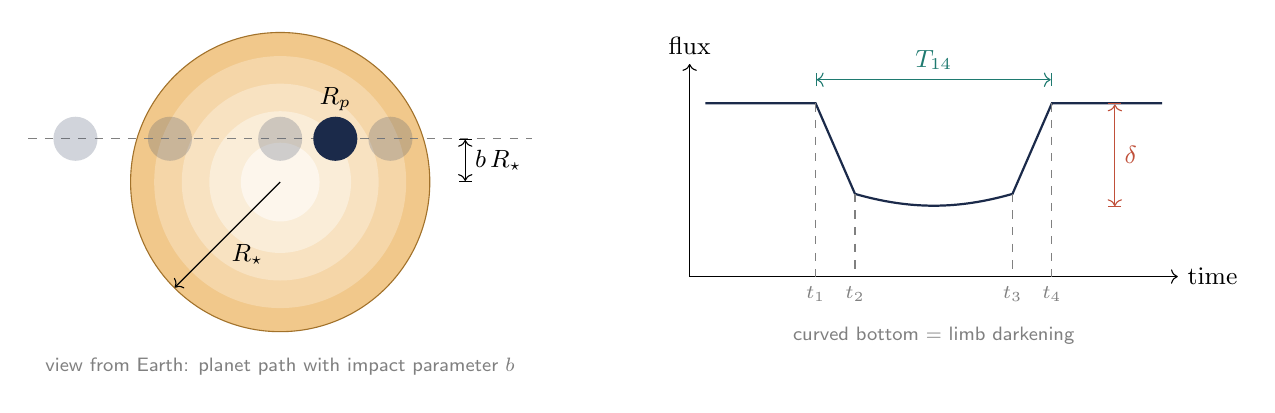
\begin{tikzpicture}[scale=1.0]
  % star disc with limb darkening rings
  \foreach \r/\c in {1.9/60,1.6/45,1.25/32,0.9/20,0.5/10}{
     \fill[amber!\c!white] (0,0) circle (\r);}
  \draw[amber!70!black] (0,0) circle (1.9);
  \draw[dashed,gray] (-3.2,0.55) -- (3.2,0.55);
  \foreach \x in {-2.6,-1.4,0,1.4} \fill[navy!80,opacity=0.25] (\x,0.55) circle (0.28);
  \fill[navy] (0.7,0.55) circle (0.28);
  \draw[|<->|,thin] (2.35,0) -- (2.35,0.55) node[midway,right,font=\small] {$b\,R_\star$};
  \draw[->,thin] (0,0) -- (-1.34,-1.34) node[midway,below right,font=\small,xshift=-2pt] {$R_\star$};
  \node[font=\small] at (0.7,1.05) {$R_p$};
  \node[font=\sffamily\scriptsize,align=center,text=gray] at (0,-2.35) {view from Earth: planet path with impact parameter $b$};
  % light curve
  \begin{scope}[xshift=5.2cm,yshift=-1.2cm]
    \draw[->] (0,0) -- (6.2,0) node[right,font=\small]{time};
    \draw[->] (0,0) -- (0,2.7) node[above,font=\small]{flux};
    \draw[thick,navy] (0.2,2.2) -- (1.6,2.2) -- (2.1,1.05) .. controls (2.8,0.85) and (3.4,0.85) .. (4.1,1.05) -- (4.6,2.2) -- (6,2.2);
    \draw[dashed,gray] (1.6,2.2) -- (1.6,0) node[below,font=\scriptsize]{$t_1$};
    \draw[dashed,gray] (2.1,1.05) -- (2.1,0) node[below,font=\scriptsize]{$t_2$};
    \draw[dashed,gray] (4.1,1.05) -- (4.1,0) node[below,font=\scriptsize]{$t_3$};
    \draw[dashed,gray] (4.6,2.2) -- (4.6,0) node[below,font=\scriptsize]{$t_4$};
    \draw[|<->|,brick] (5.4,2.2) -- (5.4,0.88) node[midway,right,font=\small]{$\delta$};
    \draw[|<->|,teal] (1.6,2.5) -- (4.6,2.5) node[midway,above,font=\small]{$T_{14}$};
    \node[font=\sffamily\scriptsize,text=gray,align=center] at (3.1,-0.75) {curved bottom = limb darkening};
  \end{scope}
\end{tikzpicture}
\end{center}

\paragraph{Depth.} If the star were a uniformly bright disc, the fraction of light blocked would be the ratio of areas:
\begin{equation}
  \delta \simeq \left(\frac{R_p}{R_\star}\right)^2 \equiv k^2 .
  \label{eq:depth}
\end{equation}
Earth crossing the Sun gives \(\delta \approx 84\) ppm; Jupiter gives about 1\%. So to measure a planet's radius you
need the star's radius, which comes from a catalogue: \(R_p = k\,R_\star\).

\paragraph{Period and orbit.} Transits repeat every orbital period \(P\). Kepler's third law gives the orbital distance:
\begin{equation}
  a^3 = \frac{G M_\star P^2}{4\pi^2}.
\end{equation}

\paragraph{Duration.} For a circular orbit with impact parameter \(b = (a/R_\star)\cos i\)~\citep{Winn2010}:
\begin{equation}
  T_{14} = \frac{P}{\pi}\arcsin\!\left[\frac{R_\star}{a}\,\frac{\sqrt{(1+k)^2-b^2}}{\sin i}\right]
  \;\approx\; 13\,\mathrm{h}\,\left(\frac{P}{365\,\mathrm{d}}\right)^{1/3}\left(\frac{\rho_\star}{\rho_\odot}\right)^{-1/3}
  \quad(b=0).
  \label{eq:duration}
\end{equation}
Short-period planets have short transits (Kepler-10\,b: under 2 hours). This matters when you choose a detrending window.

\paragraph{Stellar density for free.} Combining \(P\) and \(a/R_\star\) (which the transit shape constrains) gives the
star's mean density~\citep{SeagerMallenOrnelas2003}:
\begin{equation}
  \rho_\star = \frac{3\pi}{G P^2}\left(\frac{a}{R_\star}\right)^3 .
  \label{eq:rho}
\end{equation}
Comparing this with the catalogue density is a strong sanity check; in Week~3 we use it the other way round, as a prior.

\paragraph{Transit probability.} Only orbits seen nearly edge-on transit. For a random orientation,
\(p_\text{tr} \approx R_\star/a\): 0.47\% for an Earth--Sun analogue, \(\sim\)10\% for a hot Jupiter.
Every transit survey misses most planets for purely geometric reasons. Keep that in mind in Week~4.

\subsection{Limb darkening}
Stars are brighter at the centre of their disc than at the edge (the ``limb''), because at the edge we see higher,
cooler layers. A common description is the quadratic law with \(\mu = \cos\theta\):
\begin{equation}
  \frac{I(\mu)}{I(1)} = 1 - u_1(1-\mu) - u_2(1-\mu)^2 .
\end{equation}
A planet crossing the bright centre blocks \emph{more} than its area fraction, so Eq.~\eqref{eq:depth} under-predicts the depth
by \(\sim\)15--30\% depending on the star~\citep{Heller2019}. For a Sun-like star in the Kepler band
(\(u_1\approx0.4,\,u_2\approx0.25\)) a central transit is \(\sim\)20\% deeper than \(k^2\). Physical models
(Mandel \& Agol~\citep{MandelAgol2002}, implemented in \pkg{batman}~\citep{Kreidberg2015}) include this. Coefficients for a
given star come from tables by Claret~\citep{Claret2011,Claret2017}.

\subsection{Light curves and noise}
\label{sec:noise}
A light curve is a table of \emph{time}, \emph{flux} and \emph{flux error}. Things to know:
\begin{itemize}
  \item \textbf{SAP} flux sums the pixels in an aperture. \textbf{PDCSAP} flux has been cleaned of most spacecraft
        systematics by the mission pipeline~\citep{Jenkins2010}. Use PDCSAP for planet searches.
  \item \textbf{Cadence:} Kepler long cadence 29.4\,min, short cadence 58.8\,s. TESS: 2-min (and 20-s) targets; full-frame images
        (FFIs) every 30\,min (2018--20), 10\,min (2020--22), 200\,s (2022 on).
  \item \textbf{Time systems:} BKJD \(=\) BJD\(-2454833\) (Kepler), BTJD \(=\) BJD\(-2457000\) (TESS).
  \item \textbf{Segments:} Kepler observed in \(\sim\)90-day \emph{quarters}, TESS in 27.4-day \emph{sectors} (two 13.7-day orbits with a gap).
  \item \textbf{Noise:} photon noise, stellar granulation and spots, and instrument residuals. Kepler quoted its noise as
        \emph{CDPP} (combined differential photometric precision) over 6.5\,h, in ppm.
\end{itemize}

\begin{keyidea}
A dip with depth \(\delta\), observed in \(N\) points with scatter \(\sigma\) each, has a signal-to-noise ratio of about
\[
  \mathrm{SNR} \approx \frac{\delta}{\sigma}\sqrt{N_\text{in-transit}}, \qquad
  N_\text{in-transit} \approx N_\text{transits}\times\frac{T_{14}}{\Delta t}.
\]
Folding on the period stacks every transit, which is why we can find dips far smaller than the noise in one point. This
formula predicts most of what you will see in Week~4.
\end{keyidea}

\subsection{Detrending}
\label{sec:detrend}
Stars vary (rotation, spots, pulsations) and spacecraft drift. We estimate a smooth \emph{trend} with a sliding window that is
\textbf{longer than a transit} but \textbf{shorter than the variability}, then divide it out. Hippke et al.\ compared many methods on
Kepler, K2 and TESS data and found a time-windowed \emph{biweight} (a robust average that ignores outliers such as
transits) works best~\citep{Hippke2019wotan}. A good default window is about three times the longest transit you are
looking for. Two consequences you will measure yourself:
\begin{itemize}
  \item A window that is too short partly fits the transit and makes it shallower, or erases it.
  \item Even a robust window is pulled down by the in-transit points when the star is brightening or fading. So once a planet
        is found, \textbf{mask its transits and detrend again} before measuring the depth (\texttt{detrend.flatten\_masked}).
\end{itemize}

\subsection{Box Least Squares}
\label{sec:bls}
BLS~\citep{Kovacs2002} models a transit as a box: flux drops by \(\delta\) for duration \(D\) once per period \(P\), with phase \(t_0\).
For each trial \((P, D, t_0)\) it measures how much better a box fits than a flat line. For a box covering a (weighted)
fraction \(r\) of the points, with summed mean-subtracted in-box flux \(s\), the signal residue is
\begin{equation}
  \mathrm{SR}(P) = \max_{D,\,t_0}\left[\frac{s^2}{r(1-r)}\right]^{1/2},
\end{equation}
and the depth estimate is the difference between the mean out-of-box and in-box flux. Plotting the best value against \(P\)
gives the \textbf{BLS periodogram}. Things to understand:
\begin{itemize}
  \item \textbf{Period grid.} Trial frequencies must be spaced finely enough that, across the whole data span \(B\), the phase drifts by
        less than a fraction of a transit: \(\Delta f \lesssim D_\text{min}/B^2\) \citep{Ofir2014}. Long data sets need huge grids.
  \item \textbf{Aliases.} Folding at \(2P\) or \(P/2\) also stacks transits, so peaks appear at simple ratios of the true period.
  \item \textbf{Detection statistics.} Our code reports the SNR of the depth and the \emph{signal detection efficiency}
        SDE \(= (\text{peak} - \text{mean})/\text{std}\) of the periodogram. A threshold around 7--9 is common. Kepler used a
        multiple-event statistic (MES) threshold of 7.1\(\sigma\)~\citep{Jenkins2010,Twicken2016}. \emph{No threshold is magic}:
        Week~4 measures what yours means.
  \item \textbf{Alternatives.} Transit Least Squares (TLS) uses a limb-darkened template instead of a box and is somewhat more
        sensitive to small planets~\citep{HippkeHeller2019}. Neural-network classifiers can vet candidates~\citep{ShallueVanderburg2018}.
\end{itemize}

\subsection{Fitting a transit and its uncertainties}
\label{sec:fitting}
Given a model \(m(t;\boldsymbol\theta)\) and data \(f_i\pm\sigma_i\), least squares minimises
\(\chi^2 = \sum_i [f_i - m(t_i;\boldsymbol\theta)]^2/\sigma_i^2\). Near the minimum, the parameter covariance is
\(\mathbf{C} \approx s^2(\mathbf{J}^\mathsf{T}\mathbf{J})^{-1}\) with \(\mathbf{J}\) the Jacobian and \(s^2\) the reduced \(\chi^2\).
Read Hogg, Bovy \& Lang~\citep{Hogg2010} before trusting any error bar.

\begin{itemize}
  \item \textbf{Trapezoid model} (four parameters: \(t_0,\ \delta,\ T_{14},\ \tau\)). Robust, no dependencies, biased slightly by limb darkening.
  \item \textbf{batman model} (\(t_0,\ k,\ a/R_\star,\ b\), fixed limb darkening). Physical. At modest SNR \(b\) and \(k\) are
        \emph{degenerate}: a big planet grazing the limb looks like a small one crossing the centre. A prior on \(\rho_\star\)
        (Eq.~\ref{eq:rho}) from the catalogue breaks the degeneracy.
  \item \textbf{Long cadence smears} ingress and egress; integrate the model over the exposure (supersampling).
  \item \textbf{Error propagation} for the radius:
  \begin{equation}
    \left(\frac{\sigma_{R_p}}{R_p}\right)^2 = \left(\frac{\sigma_k}{k}\right)^2 + \left(\frac{\sigma_{R_\star}}{R_\star}\right)^2,
    \qquad \frac{\sigma_k}{k} = \frac12\frac{\sigma_\delta}{\delta}.
  \end{equation}
  For bright Kepler stars the star often dominates the error. That is why the radius gap in small planets~\citep{Fulton2017}
  was only seen after stellar radii improved.
  \item \textbf{MCMC} (\pkg{emcee}~\citep{ForemanMackey2013}; see~\citep{HoggForemanMackey2018}) maps the full posterior and gives
        honest, possibly asymmetric, error bars.
\end{itemize}

\subsection{Injection--recovery, completeness and occurrence rates}
\label{sec:injrec}
Suppose your search of a star returns nothing. Is there no planet, or could your pipeline not see it? You cannot tell from the
null result. So you test the pipeline on signals whose answer you know:
\begin{enumerate}
  \item take the \textbf{raw} light curve (before detrending, so detrending losses are included);
  \item multiply in a synthetic transit with known \(P\), \(R_p\), \(t_0\);
  \item run the identical pipeline \textbf{blind};
  \item call it \emph{recovered} if the found period and phase match (and the statistic passes your threshold);
  \item repeat thousands of times across a grid of \((P, R_p)\).
\end{enumerate}
The recovered fraction \(\eta(P,R_p)\) in each cell is the \textbf{detection efficiency} or \textbf{completeness}. With \(n\)
injections and fraction \(\hat\eta\), the binomial uncertainty is \(\sigma_\eta = \sqrt{\hat\eta(1-\hat\eta)/n}\).

Plotted against expected SNR, \(\eta\) rises from 0 to 1 along an S-shaped curve. The Kepler team measured exactly this
curve with large injection campaigns at the pixel and flux level~\citep{Christiansen2013,Christiansen2015,Christiansen2016,Christiansen2020},
reaching \(\gtrsim\)90\% recovery for strong signals. Independent teams did the same with their own pipelines, for example
Petigura et al.~\citep{Petigura2013} for Sun-like stars and Dressing \& Charbonneau~\citep{Dressing2015} for M dwarfs.
That is the closest professional analogue to this project.

\paragraph{Why it matters: occurrence rates.} If you search \(N_\star\) stars and detect planets \(j=1\ldots N_\text{det}\) in some
range of size and period, a simple estimate of how many planets each star has in that range is
\begin{equation}
  f_\text{occ} \approx \frac{1}{N_\star}\sum_{j=1}^{N_\text{det}} \frac{1}{\eta_j\,p_{\text{tr},j}},
\end{equation}
where each detection is up-weighted by how hard it was to find (\(\eta_j\)) and how unlikely its orbit was to transit
(\(p_{\text{tr},j}\)). Without \(\eta\), you cannot do this. Rigorous versions are in~\citep{Burke2015,Thompson2018}.

\paragraph{Reliability is the other half.} Completeness asks ``how many real planets did we miss?''. Reliability asks ``how many
detections are fake?''. False alarms come from noise and systematics; astrophysical false positives come from eclipsing binaries.
Kepler estimated false alarms by searching \emph{inverted} and \emph{scrambled} light curves, which cannot contain real
transits~\citep{Thompson2018}. That is a good Going Further task.

% =========================================================================
\section{Setup and tools}
\label{sec:setup}

\subsection{Option A: Google Colab (zero install, recommended for Week 1)}
\begin{enumerate}
  \item Fork the project repository on GitHub (button top right), so you have your own copy.
  \item Open a notebook from the \texttt{notebooks/} folder via its ``Open in Colab'' badge.
  \item In the first cell, change \texttt{REPO\_URL} to your fork and run it. It clones the repo and installs packages
        (\(\sim\)1\,min). Colab forgets everything after a disconnect: rerun the first cell.
  \item Save your work back to GitHub: \emph{File \(\to\) Save a copy in GitHub}.
\end{enumerate}

\subsection{Option B: your own computer (recommended from Week 2)}
\begin{code}
git clone https://github.com/<you>/exoplanet-transit-winter-project.git
cd exoplanet-transit-winter-project
# conda users:
conda env create -f environment.yml
conda activate exotransit
# (no conda? python -m venv .venv, activate it, then: pip install -r requirements.txt)
pip install -e .                         # makes `import transitpipe` work everywhere
pytest -q                                # all tests should pass (offline, ~10 s)
python scripts/run_baseline.py --synthetic
jupyter lab
\end{code}

\subsection{What is in the repository}
\begin{center}
\footnotesize
\begin{tabularx}{\linewidth}{@{}L{5.2cm} Y@{}}
\toprule
\textbf{Path} & \textbf{What it is}\\
\midrule
\texttt{notebooks/00\ldots04\_*.ipynb} & One notebook per milestone, with explanations, exercises (\emph{Your turn}) and checkpoints.\\
\texttt{src/transitpipe/io.py} & \texttt{LightCurve} container; download from MAST via Lightkurve; CSV in/out.\\
\texttt{src/transitpipe/detrend.py} & Median / Savitzky--Golay / biweight detrending, gap handling, sigma clipping, transit masks.\\
\texttt{src/transitpipe/search.py} & BLS wrapper (astropy), period grid, SDE/SNR, multi-planet search, alias matching.\\
\texttt{src/transitpipe/fit.py} & Trapezoid and batman fits, error bars, stellar-density prior, bootstrap.\\
\texttt{src/transitpipe/inject.py} & Synthetic light curves, transit injection, the injection--recovery engine, completeness maps.\\
\texttt{src/transitpipe/plotting.py} & Raw/trend, periodogram, folded transit, efficiency-curve plots.\\
\texttt{scripts/run\_baseline.py} & Whole baseline pipeline from the command line.\\
\texttt{scripts/run\_injection\_recovery.py} & Whole injection--recovery experiment from the command line (parallel).\\
\texttt{tests/test\_pipeline.py} & Tests that encode physics facts and an end-to-end recovery.\\
\texttt{docs/} & This guide, its bibliography, \texttt{RESOURCES.md}, and a report template.\\
\bottomrule
\end{tabularx}
\end{center}

\begin{keyidea}
The package is deliberately short and readable. Each notebook first makes you build a step \emph{by hand} (a slow loop),
then shows the package version and checks they agree. Read the source in \texttt{src/transitpipe/}; it is written to be read.
\end{keyidea}

\subsection{Getting data from MAST}
\begin{code}
import lightkurve as lk
sr = lk.search_lightcurve("Kepler-10", mission="Kepler", author="Kepler", exptime="long")
lc = sr[2:4].download_all().stitch()          # two quarters, each normalised, joined
# or with our wrapper (plain NumPy arrays inside):
from transitpipe import io
lc = io.get_lightcurve("Kepler-10", mission="Kepler", exptime="long", quarter=[3, 4])
\end{code}
\begin{itemize}
  \item Filter searches with \texttt{author} (\texttt{"Kepler"}, \texttt{"SPOC"}, \texttt{"QLP"}, \texttt{"TESS-SPOC"}), \texttt{exptime},
        \texttt{quarter}, \texttt{sector}. TESS FFI cut-outs for stars without 2-min data: \texttt{lk.search\_tesscut}.
  \item Lightkurve caches downloads (\texttt{\textasciitilde/.lightkurve/cache}); a second download is instant. MAST is sometimes slow
        or down: download your target early, not the night before a deadline.
  \item Look up stellar parameters in the NASA Exoplanet Archive (Kepler) or ExoFOP-TESS (TIC values).
\end{itemize}

% =========================================================================
\section{The four-week plan}
\label{sec:plan}

Each week lists: goals, a session-by-session plan with time estimates, the checkpoint, reading, pitfalls, and the Going
Further box. Hours are a guide for the core track. Notebook numbers refer to \texttt{notebooks/}.

% ------------------------------------------------------------------ WEEK 1 --
\newpage
\weekbanner{1}{Foundations}{Python from zero, the transit method, and your first real light curve}

\textbf{Goals.} Everyone can run Python in a notebook, use NumPy arrays and boolean masks, make labelled plots and use
Git. Everyone understands why a transit's depth gives the planet's size. Everyone has downloaded and plotted a real
Kepler light curve and chosen a personal target.

\begin{center}
\small
\begin{tabularx}{\linewidth}{@{}L{2.4cm} Y l@{}}
\toprule
\textbf{When} & \textbf{Task} & \textbf{Hours}\\
\midrule
Session A & \textbf{Kick-off.} Talk: exoplanets, the transit method, Kepler and TESS (30\,min). Live demo: a Kepler-10 light curve
in Colab in 5\,minutes. Everyone: GitHub account, fork the repo, open Notebook~00. & \hrs{2}\\
Self & \textbf{Notebook 00: Python crash course.} Variables, functions, NumPy, boolean masks, Matplotlib; build a fake transit and
fold it. Juniors/seniors: skim and help. & \hrs{3--4}\\
Self & \textbf{Git basics.} Software Carpentry \emph{Version Control with Git}, episodes 1--7 (or GitHub Skills ``Introduction to GitHub'').
Make your first commit: a README with your name and goal. & \hrs{1}\\
Self & \textbf{Reading.} NASA ``What is the transit method?''; Section~\ref{sec:geometry}--\ref{sec:noise} of this guide; Winn (2010) \S1--2 (skim). & \hrs{1--2}\\
Session B & \textbf{Notebook 01: real data.} MAST search, SAP vs PDCSAP, quality flags, our \texttt{LightCurve} class.
\textbf{Choose your own target} (Section~\ref{sec:targets}) and record stellar parameters. & \hrs{2--3}\\
Self & Finish Notebook 01 on your target. Start \texttt{LOG.md}. Commit. & \hrs{1--2}\\
\midrule
 & \textbf{Total} & \textbf{10--14}\\
\bottomrule
\end{tabularx}
\end{center}

\begin{checkpoint}
\begin{checklist}
  \item Your fork exists, has a README stating your target, and Notebooks~00 and~01 run top to bottom.
  \item \emph{Your turn} answers written in your own words (markdown cells).
  \item A labelled plot of your target's raw light curve, saved in \texttt{figures/}.
  \item A table in your README: star name, \(R_\star\pm\sigma\), \(M_\star\pm\sigma\), published planet \(P\) and \(R_p\), with sources.
\end{checklist}
\end{checkpoint}

\begin{reading}
Core: NASA Exoplanet Exploration, \emph{Ways to find a planet}; Section~\ref{sec:geometry}--\ref{sec:noise};
Lightkurve tutorial \emph{Searching \& downloading data}. Extra: Winn~\citep{Winn2010} \S1--2;
Haswell~\citep{Haswell2010} ch.\,1--2; Borucki et al.~\citep{Borucki2010}; Ricker et al.~\citep{Ricker2015}.
\end{reading}

\begin{pitfall}
\begin{itemize}
  \item Colab disconnected and ``nothing works'': rerun the setup cell (Runtime \(\to\) Run all).
  \item Plotting \texttt{time} in BKJD or BTJD and comparing it to a published ephemeris in BJD: add the offset.
  \item Stitching quarters without normalising each one first gives jumps between quarters.
  \item Committing \texttt{.fits} files (tens of MB). They are git-ignored; keep it that way.
\end{itemize}
\end{pitfall}

\begin{goingfurther}
\begin{itemize}
  \item \textbf{Noise vs brightness.} Use \texttt{lc.estimate\_cdpp()} on 20--30 Kepler stars of different magnitudes and plot CDPP vs
        Kepler magnitude. Explain the shape: where does photon noise dominate?
  \item \textbf{Write the physics yourself.} Implement depth \(\to\) radius, Kepler's third law and Eq.~\eqref{eq:duration} from scratch
        with \pkg{pytest} tests (compare with \texttt{tests/test\_pipeline.py}).
  \item \textbf{All of Kepler-10.} Download all 15+ quarters, stitch them, and look for Kepler-10\,c (\(P\approx45\)\,d) by eye.
  \item \textbf{Quality flags.} Decode the \texttt{QUALITY} bitmask; plot which cadences are flagged and why.
\end{itemize}
\end{goingfurther}

% ------------------------------------------------------------------ WEEK 2 --
\newpage
\weekbanner{2}{Find it}{Detrending and the Box Least Squares search}

\textbf{Goals.} Understand and control detrending; understand BLS well enough to code a slow version yourself;
recover Kepler-10\,b blind from raw data; search your own target and interpret its periodogram, including aliases.

\begin{center}
\small
\begin{tabularx}{\linewidth}{@{}L{2.4cm} Y l@{}}
\toprule
\textbf{When} & \textbf{Task} & \textbf{Hours}\\
\midrule
Session A & \textbf{Lecture:} noise, detrending windows, robust statistics (median vs mean); BLS on the whiteboard; periodograms and aliases.
Live: code the sliding-median detrender together. & \hrs{2}\\
Self & \textbf{Notebook 02 \S1:} hand-made detrender vs package; the window-length experiment on synthetic data; compare median/savgol/biweight. & \hrs{2--3}\\
Self & \textbf{Notebook 02 \S2--3:} BLS by hand (slow loop), then \texttt{astropy} BLS; recover Kepler-10\,b; fold and inspect. & \hrs{2--3}\\
Self & \textbf{Reading:} Kov\'acs et al.~\citep{Kovacs2002} \S1--2; Hippke et al.~\citep{Hippke2019wotan} \S1--3; Lightkurve tutorial
\emph{Identifying transiting planet signals}. & \hrs{1--2}\\
Session B & \textbf{Run on your target.} Lightning round: every student shows one periodogram in 2 minutes and explains the tallest peak. & \hrs{2--3}\\
Self & Write up: a table of (window, depth, noise) and your BLS result table; commit figures; update \texttt{LOG.md}. & \hrs{1}\\
\midrule
 & \textbf{Total} & \textbf{10--14}\\
\bottomrule
\end{tabularx}
\end{center}

A minimal pass of the pipeline looks like this (the notebook does it step by step):
\begin{code}
from transitpipe import io, detrend, search, plotting
lc   = io.get_lightcurve("Kepler-10", mission="Kepler", exptime="long", quarter=[3, 4])
flat = detrend.sigma_clip(detrend.flatten(lc, method="median", window_days=0.5))
res  = search.bls(flat, min_period=0.5, max_period=10)
print(res.summary())          # P = 0.8377 d | depth ~ 150 ppm | SNR ~ 80 | SDE ~ 30
plotting.plot_periodogram(res); plotting.plot_fold(flat, res.period, res.t0)
\end{code}

\begin{checkpoint}
\begin{checklist}
  \item Kepler-10\,b recovered: periodogram and folded transit committed, period within 0.1\% of 0.83749\,d.
  \item Your own target: periodogram, fold, and a table of \(P\), depth, SNR, SDE compared with the published period.
  \item One paragraph explaining how the detrending window changed the measured depth, with your table.
\end{checklist}
\end{checkpoint}

\begin{pitfall}
\begin{itemize}
  \item \textbf{Window too short} for your planet's transit: the dip shrinks or vanishes. Use \(\gtrsim3\times T_{14}\).
  \item \textbf{Symmetric sigma clipping} deletes transits (they are low outliers). Clip upward only.
  \item \textbf{BLS on raw flux} finds stellar rotation, not planets.
  \item \textbf{Grid limits:} periods longer than half the baseline cannot show two transits; ultra-short periods below
        \texttt{min\_period} (e.g.\ LHS~3844\,b, \(P=0.46\)\,d) are never tried.
  \item \textbf{Aliases:} a peak at exactly \(2P\) or \(P/2\) of the published value is not a new planet.
  \item \textbf{TESS momentum dumps} every few days create periodic glitches that BLS loves. Check flagged cadences.
\end{itemize}
\end{pitfall}

\begin{goingfurther}
\begin{itemize}
  \item \textbf{Fast BLS from scratch.} Vectorise the hand BLS with NumPy (or \pkg{numba}); time it against astropy.
  \item \textbf{Multi-planet systems.} \texttt{search.search\_multiple} masks each detection and searches again. Try TOI-270 (three
        planets, TESS) or Kepler-11 (six planets).
  \item \textbf{TLS vs BLS.} Install \pkg{transitleastsquares}~\citep{HippkeHeller2019}; compare SDE for a small planet.
  \item \textbf{Vetting.} Odd/even depth test and a search for a secondary eclipse at phase 0.5. Either failing suggests an
        eclipsing binary. Apply both to Kepler-10\,b and to a known eclipsing binary.
  \item \textbf{Long periods.} Search all quarters of Kepler-22 for its 290-day planet: three transits in four years.
\end{itemize}
\end{goingfurther}

% ------------------------------------------------------------------ WEEK 3 --
\newpage
\weekbanner{3}{Measure it}{Transit fitting, error bars, and the planet's radius}

\textbf{Goals.} Measure the planet's radius with a defensible uncertainty, understand where that uncertainty comes from,
and compare the result with published values. Begin the written report.

\begin{center}
\small
\begin{tabularx}{\linewidth}{@{}L{2.4cm} Y l@{}}
\toprule
\textbf{When} & \textbf{Task} & \textbf{Hours}\\
\midrule
Session A & \textbf{Lecture:} geometry (\(\delta,\ T_{14},\ b,\ a/R_\star\)), limb darkening, \(\chi^2\) and least squares, covariance,
error propagation, what MCMC does (intuition only). & \hrs{2}\\
Self & \textbf{Notebook 03 \S1--3:} quick estimate from the BLS depth; two-pass (masked) detrending; trapezoid fit; error propagation;
bootstrap check. & \hrs{3}\\
Self & \textbf{Notebook 03 \S4:} batman fit with limb darkening, supersampling and a stellar-density prior. Look up limb-darkening
coefficients for your star. & \hrs{2--3}\\
Session B & \textbf{Group figure:} each student adds their planet to a club radius--period diagram over the known population
(NASA Exoplanet Archive). Discuss disagreements with the literature. & \hrs{2--3}\\
Self & \textbf{Write:} first draft of the Data and Methods sections (\(\sim\)1 page) using \texttt{docs/report\_template.tex}. & \hrs{2}\\
\midrule
 & \textbf{Total} & \textbf{11--13}\\
\bottomrule
\end{tabularx}
\end{center}

\begin{code}
from transitpipe import detrend, fit, utils
# pass 2: re-detrend with the transits hidden, then fit
flat2 = detrend.flatten_masked(lc, res.period, res.t0, res.duration,
                               window_days=0.5)
flat2 = detrend.sigma_clip(flat2)
star = dict(rstar_rsun=1.065, rstar_err=0.009)
ft = fit.fit_single_transit(flat2, res, model="trapezoid", **star)

rho, rho_err = utils.stellar_density(1.065, 0.910, 0.009, 0.021)
fb = fit.fit_single_transit(flat2, res, model="batman", **star,
                            rho_star=rho, rho_star_err=rho_err,
                            u=(0.40, 0.26), exptime_days=0.0204)
print(ft.summary()); print(fb.summary())
\end{code}

\begin{checkpoint}
\begin{checklist}
  \item Kepler-10\,b radius with uncertainty, compared with the published \(1.47\,\Rearth\)~\citep{Batalha2011}.
  \item Your target: a table of \(R_p\) from (quick BLS, trapezoid, batman, literature), with a sentence on each difference.
  \item A folded transit figure with the best-fit model and residuals.
  \item Draft Methods section committed.
\end{checklist}
\end{checkpoint}

\begin{pitfall}
\begin{itemize}
  \item \textbf{Fitting the first-pass detrended data}: depth biased low (we measured \(\sim\)25\% on an active synthetic star). Always re-detrend with transits masked.
  \item \textbf{No supersampling for long cadence}: ingress/egress too sharp, \(b\) and \(a/R_\star\) wrong.
  \item \textbf{Huge error bars on \(R_p/R_\star\)} from batman: that is the \(b\)--\(k\) degeneracy. Use the density prior.
  \item \textbf{A zero error bar} means the parameter hit a bound, not that it is perfectly measured.
  \item \textbf{TESS dilution:} 21\('' \) pixels can include light from neighbours, making transits shallower. Check the \texttt{CROWDSAP} header keyword.
  \item \textbf{Stellar radius source:} different catalogues differ by several percent; say which one you used.
\end{itemize}
\end{pitfall}

\begin{goingfurther}
\begin{itemize}
  \item \textbf{MCMC.} Run the \pkg{emcee} cell in Notebook~03; make a corner plot; compare with the covariance errors.
  \item \textbf{Fit limb darkening} with Kipping's \(q_1,q_2\) parametrisation~\citep{Kipping2013} on a high-SNR hot Jupiter (Kepler-8\,b, HAT-P-7\,b).
  \item \textbf{Ephemeris and TTVs.} Fit each transit's mid-time individually; plot observed\(-\)calculated. Try Kepler-9, which shows
        large transit-timing variations from planet--planet interactions.
  \item \textbf{Physical context.} Compute the planet's equilibrium temperature and insolation; place it on the radius gap~\citep{Fulton2017}.
  \item \textbf{Grazing transits.} Fit TrES-2\,b (Kepler-1\,b), which has a high impact parameter.
\end{itemize}
\end{goingfurther}

% ------------------------------------------------------------------ WEEK 4 --
\newpage
\weekbanner{4}{Know your limits}{Injection--recovery: measure your own pipeline's detection efficiency}

\textbf{Goals.} Measure your pipeline's completeness as a function of period and radius on synthetic and real data; summarise it
with an efficiency curve; run one controlled experiment that changes one pipeline choice; present everything.

\begin{center}
\small
\begin{tabularx}{\linewidth}{@{}L{2.4cm} Y l@{}}
\toprule
\textbf{When} & \textbf{Task} & \textbf{Hours}\\
\midrule
Session A & \textbf{Lecture:} completeness vs reliability; binomial statistics; the Kepler DR25 story; how occurrence rates use \(\eta\).
Each student writes down their recovery criteria and the one experiment they will run. & \hrs{2}\\
Self & \textbf{Notebook 04 \S1--2:} one injection by hand; the synthetic grid; completeness map; efficiency curve and \(S_{50}\). & \hrs{2}\\
Self & \textbf{Notebook 04 \S3:} the real-data grid with the known planet masked. Let it run in parallel or overnight (\texttt{scripts/run\_injection\_recovery.py}). & \hrs{1 + compute}\\
Self & \textbf{Notebook 04 \S4:} your controlled experiment (same seed, change one thing). & \hrs{3}\\
Session B & \textbf{Writing and talk workshop:} peer review of drafts in pairs; poster and slide clinic; dry runs. & \hrs{3}\\
Self & Finish report, clean repo, tag release \texttt{v1.0}. & \hrs{2--3}\\
End & \textbf{Demo Day:} 5-minute talks or posters, 2 minutes of questions each. & \hrs{2--3}\\
\midrule
 & \textbf{Total} & \textbf{13--15}\\
\bottomrule
\end{tabularx}
\end{center}

\begin{code}
python scripts/run_injection_recovery.py --synthetic --fast          # 30-second demo
python scripts/run_injection_recovery.py --target "Kepler-10" --mission Kepler --quarter 3 \
    --rstar 1.065 --mask-period 0.83766 --mask-t0 260.537 --mask-duration 0.08 \
    --method median --window 0.5 --n-per-cell 20 --n-jobs 4
\end{code}

\begin{keyidea}
\textbf{Freeze your pipeline before you measure it.} The detrending method and window, the BLS grid and the detection threshold used
for injections must be the ones you used for the real search. If you change the pipeline, you must re-measure its completeness.
\end{keyidea}

\paragraph{Experiment menu} (choose one; seniors choose two):
\begin{enumerate}
  \item \textbf{Detrending window:} 0.25, 0.5, 1, 2\,d. Where do long-duration (long-period) planets start to be lost?
  \item \textbf{Detrending method:} median vs Savitzky--Golay vs biweight. Does the result of~\citep{Hippke2019wotan} hold for your star?
  \item \textbf{Threshold:} SDE 6 vs 7 vs 9, together with the number of false alarms on light curves with no injection.
  \item \textbf{Period-grid density:} \texttt{oversample} 0.5 vs 1 vs 3. Does a coarse grid miss planets? Which ones?
  \item \textbf{Kepler vs TESS:} one Kepler quarter vs one TESS sector for stars of similar brightness.
  \item \textbf{Quiet vs active star:} how much completeness does stellar variability cost?
\end{enumerate}

\begin{checkpoint}
\begin{checklist}
  \item Completeness maps (synthetic and real) with the number of injections per cell stated.
  \item Efficiency curve with your \(S_{50}\) (the SNR at which you find half the planets).
  \item One controlled experiment with a one-sentence conclusion supported by a figure.
  \item Final report (Section~\ref{sec:deliverables}), repo tagged \texttt{v1.0}, talk or poster delivered.
\end{checklist}
\end{checkpoint}

\begin{pitfall}
\begin{itemize}
  \item \textbf{Injecting after detrending.} Then you never measure the losses that detrending causes.
  \item \textbf{Leaving the real planet in.} The pipeline keeps finding it instead of your fake one. Mask it first (and try once without, to see).
  \item \textbf{Too few injections.} With 5 per cell, \(\sigma_\eta\) can be 0.2. Report it.
  \item \textbf{Calling aliases recoveries} without saying so. Our code logs them separately (\texttt{match\_kind}).
  \item \textbf{Not fixing the random seed}: results you cannot reproduce.
\end{itemize}
\end{pitfall}

\begin{goingfurther}
\begin{itemize}
  \item \textbf{Scale up.} 20--50 injections per cell on a finer grid using a lab machine or the university cluster (\texttt{-{}-n-jobs}).
  \item \textbf{Reliability.} Run the pipeline on inverted (\(2-f\)) and time-scrambled light curves (no real transits possible) and count
        detections above threshold. Combine with completeness to choose an optimal threshold.
  \item \textbf{A mini occurrence-rate study.} Search 50--200 TESS stars of one type, measure completeness per star, and estimate an
        occurrence rate for one bin with the inverse-detection-efficiency formula. Compare with Dressing \& Charbonneau~\citep{Dressing2015} (M dwarfs).
  \item \textbf{Gamma-CDF efficiency model} as in Christiansen et al.~\citep{Christiansen2015} instead of our logistic.
  \item \textbf{Limb-darkened injections} (\texttt{model="batman"}). Does completeness change for a box-shaped search?
\end{itemize}
\end{goingfurther}

% =========================================================================
\section{Deliverables and assessment}
\label{sec:deliverables}

\subsection{1. The repository}
Your repo is the thing people will click on from your résumé. The README must contain: a one-paragraph summary with your
headline numbers, a figure, how to reproduce the results (exact commands), and credits. All notebooks run top to bottom;
\texttt{pytest} passes; no data files; a \texttt{v1.0} release.

\subsection{2. The report (4--6 pages)}
Use \texttt{docs/report\_template.tex} (or the free AASTeX template on Overleaf). Sections:
\begin{enumerate}
  \item \textbf{Abstract} (\(\le\)150 words, with your main numbers).
  \item \textbf{Introduction}: transit method, why completeness matters, what you did.
  \item \textbf{Data}: mission, target(s), sectors/quarters, cadence, flux type, stellar parameters and sources.
  \item \textbf{Methods}: detrending, search, fitting, injection--recovery, with every parameter value.
  \item \textbf{Results}: periodogram, fold with model, radius table, completeness map, efficiency curve.
  \item \textbf{Discussion}: comparison with literature; what limits your pipeline; what you would do next.
  \item \textbf{References}: at least the data source, the software you used~\citep{Lightkurve2018,Astropy2022} and the papers you compared with.
\end{enumerate}

\subsection{3. The talk (5 min) or poster}
Five slides is enough: the question; the data; the found planet and its radius; the completeness map; the one thing you learned.
One idea per slide, big figures, axis labels readable from the back of the room.

\subsection{Rubric}
\begin{center}
\small
\begin{tabularx}{\linewidth}{@{}L{3.2cm} c Y Y@{}}
\toprule
\textbf{Criterion} & \textbf{Pts} & \textbf{Meets expectations} & \textbf{Excellent}\\
\midrule
Baseline science & 25 & Planet recovered; radius with an error bar; compared with literature. & Two-pass detrending justified; batman with prior; disagreements explained physically.\\
Injection--recovery & 25 & Completeness map and efficiency curve, recovery criteria stated. & Controlled experiment with error bars and a clear, supported conclusion.\\
Code \& reproducibility & 20 & Repo runs; README with commands; regular commits. & Own module or tests added; clean, documented, release tagged.\\
Report & 20 & All sections present; labelled figures; sources cited. & Reads like a short paper; every number traceable to code.\\
Talk / poster & 10 & Clear, on time. & Tells a story; handles questions well.\\
\bottomrule
\end{tabularx}
\end{center}

% =========================================================================
\clearpage
\section{Suggested targets}
\label{sec:targets}

Everyone starts with \textbf{Kepler-10\,b} (shared answer key). Then each student picks one personal target. Values below are
approximate, for orientation only: \textbf{look up current values in the NASA Exoplanet Archive and cite them.}

\begin{center}
\small
\begin{tabularx}{\linewidth}{@{}l l c c c l Y@{}}
\toprule
\textbf{Planet} & \textbf{Data} & \(P\) [d] & \(R_p\) & \(\delta\) & \textbf{Level} & \textbf{What it teaches}\\
\midrule
\multicolumn{7}{@{}l}{\textit{Hot Jupiters: easy detections, beautiful fits}}\\
Kepler-8\,b & Kepler & 3.52 & 1.4\,\(R_J\) & \(\sim\)0.9\% & \(\star\) & First clean fit; limb darkening is obvious.\\
HAT-P-7\,b & Kepler & 2.20 & 1.4\,\(R_J\) & \(\sim\)0.6\% & \(\star\) & Going further: secondary eclipse and phase curve.\\
TrES-2\,b & Kepler & 2.47 & 1.2\,\(R_J\) & \(\sim\)1.4\% & \(\star\star\) & Grazing orbit (\(b\approx0.85\)): \(b\)--\(k\) degeneracy.\\
WASP-18\,b & TESS & 0.94 & 1.2\,\(R_J\) & \(\sim\)1\% & \(\star\) & TESS 2-min data; massive, very close-in planet.\\
\multicolumn{7}{@{}l}{\textit{Small planets: the real challenge}}\\
Kepler-10\,b & Kepler & 0.837 & 1.47\,\(\Rearth\) & \(\sim\)150\,ppm & \(\star\star\) & Shared target. Rocky, hot, many transits.\\
\(\pi\)~Men\,c & TESS & 6.27 & 2.0\,\(\Rearth\) & \(\sim\)300\,ppm & \(\star\star\) & Very bright star; first TESS planet~\citep{Huang2018}.\\
LHS~3844\,b & TESS & 0.46 & 1.3\,\(\Rearth\) & \(\sim\)0.4\% & \(\star\star\) & Ultra-short period: lower \texttt{min\_period}!\\
TOI-270\,b,c,d & TESS & 3.4, 5.7, 11.4 & 1.2--2.4\,\(\Rearth\) & 0.1--0.3\% & \(\star\star\star\) & M dwarf; multi-planet search.\\
AU~Mic\,b & TESS & 8.46 & \(\sim\)4\,\(\Rearth\) & \(\sim\)0.3\% & \(\star\star\star\) & Young, spotted, flaring star: detrending is hard.\\
\multicolumn{7}{@{}l}{\textit{Long periods and multiplanet systems (Going further)}}\\
Kepler-11 & Kepler & 10--118 & 1.8--4.2\,\(\Rearth\) & various & \(\star\star\star\) & Six planets; iterative search.\\
Kepler-9\,b,c & Kepler & 19.2, 39.0 & \(\sim\)0.8\,\(R_J\) & \(\sim\)0.6\% & \(\star\star\star\) & Transit-timing variations.\\
Kepler-22\,b & Kepler & 290 & 2.1--2.4\,\(\Rearth\) & \(\sim\)500\,ppm & \(\star\star\star\) & Only three transits; period-grid limits.\\
TOI-700\,d & TESS & 37.4 & 1.2\,\(\Rearth\) & \(\sim\)700\,ppm & \(\star\star\star\) & Earth-size, habitable zone; many sectors needed.\\
\bottomrule
\end{tabularx}
\end{center}

\textbf{How to choose your own:} in the
\href{https://exoplanetarchive.ipac.caltech.edu/cgi-bin/TblView/nph-tblView?app=ExoTbls&config=PSCompPars}{Planetary Systems Composite table},
filter by discovery facility (Kepler or TESS), sort by transit depth, and choose a planet with depth \(>500\)\,ppm and \(P<10\)\,d
for a first target. Check that the star has 2-min (TESS) or long-cadence (Kepler) light curves in MAST.

% =========================================================================
\section{Beyond the four weeks}
\label{sec:beyond}
\begin{itemize}
  \item \textbf{Publish a short result.} \emph{Research Notes of the AAS} (RNAAS) publishes short, citable, refereed notes (about 1{,}000
        words). A careful completeness analysis, or a well-vetted candidate, can qualify. Ask a faculty member to advise.
  \item \textbf{Observe a transit yourself.} NASA's \emph{Exoplanet Watch} trains amateurs and students to observe transits with small
        telescopes and contribute timing data. If the club has a telescope and a CCD/CMOS camera, a hot-Jupiter transit is a feasible
        first observation.
  \item \textbf{Find new planets.} \emph{Planet Hunters TESS} (Zooniverse) has led to real discoveries by volunteers. Your trained eye is now useful.
  \item \textbf{Present.} The AAS winter meeting has undergraduate poster sessions; many universities run undergraduate research symposia.
  \item \textbf{Learn the professional tools.} \pkg{exoplanet}/\pkg{PyMC} or \pkg{juliet} for joint fits, Gaussian processes (\pkg{celerite2})
        for stellar variability, \pkg{eleanor} or \pkg{TESS-Gaia Light Curve} for FFI photometry.
\end{itemize}

% =========================================================================
\section{Resource compendium}
\label{sec:resources}
Curated and annotated. \(\star\) = start here. Everything here is free unless marked.

\subsection{Start here: the transit method, gently}
\begin{reslist}
\res{\(\star\) NASA Exoplanet Exploration: Ways to find a planet}{https://science.nasa.gov/exoplanets/how-we-find-and-characterize/}{NASA's illustrated introduction to transits and the other detection methods.}
\res{\(\star\) NAAP Transit simulator (Univ.\ of Nebraska--Lincoln)}{https://astro.unl.edu/newRTs/Transits/background/Transit1.html}{Interactive: move a planet across a star and watch the light curve change. Excellent for building intuition.}
\res{OpenLearn: Introduction to exoplanets (The Open University)}{https://www.open.edu/openlearn/mod/oucontent/view.php?id=74851&section=4.1}{Free short course; transit depth, radius and limb darkening at first-year level.}
\res{HEASARC: How to find an exoplanet with TESS data}{https://heasarc.gsfc.nasa.gov/docs/tess/HowToFindAnExoplanet-UserVersion.html}{The TESS Science Support Center's own beginner notebook: data to BLS in one sitting.}
\end{reslist}

\subsection{Python, Git and scientific computing}
\begin{reslist}
\res{\(\star\) Software Carpentry: Plotting and Programming in Python}{https://swcarpentry.github.io/python-novice-gapminder/}{The best zero-to-useful Python lesson for scientists.}
\res{\(\star\) Software Carpentry: Version Control with Git}{https://swcarpentry.github.io/git-novice/}{Git from scratch, with the reasons behind each command.}
\res{NumPy: the absolute basics for beginners}{https://numpy.org/doc/stable/user/absolute_beginners.html}{Arrays, indexing, boolean masks, broadcasting.}
\res{Matplotlib quick start}{https://matplotlib.org/stable/users/explain/quick_start.html}{Figures and axes done properly, the way the notebooks use them.}
\res{Python Data Science Handbook (J.~VanderPlas)}{https://jakevdp.github.io/PythonDataScienceHandbook/}{Free online book: NumPy, pandas, Matplotlib in depth.}
\res{Learn Astropy}{https://learn.astropy.org/}{Tutorials on units, time, coordinates, FITS files and tables.}
\res{GitHub Skills}{https://skills.github.com/}{Short interactive GitHub courses (repos, pull requests, GitHub Pages).}
\res{Code/Astro workshop materials}{https://github.com/semaphoreP/codeastro}{For seniors: turning research code into a real Python package (testing, docs, packaging).}
\end{reslist}

\subsection{Data archives and catalogues}
\begin{reslist}
\res{\(\star\) MAST: Barbara A.\ Mikulski Archive for Space Telescopes}{https://archive.stsci.edu/}{Home of all Kepler, K2 and TESS data.}
\res{MAST Kepler mission page and documentation}{https://archive.stsci.edu/missions-and-data/kepler}{Data products, archive manual, data characteristics handbook (cadences, quality flags, systematics).}
\res{MAST TESS mission page}{https://archive.stsci.edu/missions-and-data/tess}{TESS products, data release notes, and the Science Data Products Description document.}
\res{\(\star\) NASA Exoplanet Archive}{https://exoplanetarchive.ipac.caltech.edu/}{Every confirmed planet with parameters and references. Your answer key and stellar parameters.}
\res{ExoFOP-TESS}{https://exofop.ipac.caltech.edu/tess/}{TESS Objects of Interest, TIC stellar parameters, and follow-up notes.}
\res{TESS Science Support Center (HEASARC)}{https://heasarc.gsfc.nasa.gov/docs/tess/}{Sector pointings, the Web TESS Viewing Tool (is my star observed?), and tutorials.}
\res{astroquery.mast documentation}{https://astroquery.readthedocs.io/en/latest/mast/mast.html}{Lower-level MAST queries when Lightkurve is not enough.}
\end{reslist}

\subsection{Hands-on tutorials and notebooks}
\begin{reslist}
\res{\(\star\) Lightkurve documentation and tutorials}{https://lightkurve.github.io/lightkurve/}{The main tool used in this project; tutorials from first light curve to planet search.}
\res{Lightkurve: Searching \& downloading Kepler, K2, and TESS data}{https://lightkurve.github.io/lightkurve/tutorials/1-getting-started/searching-for-data-products.html}{Week 1 companion to Notebook 01.}
\res{\(\star\) Lightkurve: Identifying transiting planet signals}{https://lightkurve.github.io/lightkurve/tutorials/3-science-examples/exoplanets-identifying-transiting-planet-signals.html}{BLS with Lightkurve and astropy; two planets in one system. Week 2.}
\res{Lightkurve: How to recover a known planet in Kepler data}{https://lightkurve.github.io/lightkurve/tutorials/3-science-examples/exoplanets-recover-a-known-planet.html}{Kepler-10\,b step by step; check your Week 2 result against it.}
\res{HEASARC TESS tutorial index}{https://heasarc.gsfc.nasa.gov/docs/tess/tutorial_landing.html}{Many TESS notebooks: LightCurve objects, FFIs, target pixel files.}
\res{lksearch}{https://lightkurve.github.io/lksearch/}{Newer, faster MAST search package from the Lightkurve team.}
\res{MAST notebooks}{https://spacetelescope.github.io/mast_notebooks/}{Official STScI notebooks for Kepler/TESS data access and analysis.}
\res{Astropy: Box Least Squares}{https://docs.astropy.org/en/stable/timeseries/bls.html}{Documentation of the BLS implementation used in \texttt{search.py}.}
\res{batman documentation}{https://lkreidberg.github.io/batman/docs/html/index.html}{Transit model used in Week 3; tutorial on limb-darkening laws and supersampling.}
\res{wotan (GitHub)}{https://github.com/hippke/wotan}{Detrending library with many methods; the biweight is our recommended default.}
\res{Transit Least Squares}{https://transitleastsquares.readthedocs.io/}{Alternative to BLS with a limb-darkened template; good tutorials.}
\res{emcee documentation}{https://emcee.readthedocs.io/}{MCMC sampler; the ``Fitting a model to data'' tutorial is a must.}
\res{exoplanet (PyMC) case studies}{https://docs.exoplanet.codes/}{Professional-grade joint fitting with Gaussian processes. For seniors.}
\end{reslist}

\subsection{Books and lecture notes}
\begin{reslist}
\res{\(\star\) J.\ Winn, Transits and Occultations (2010)}{https://arxiv.org/abs/1001.2010}{The standard review; every equation in this guide is in it.}
\res{C.\ Haswell, Transiting Exoplanets (CUP, 2010)}{https://www.cambridge.org/core/books/transiting-exoplanets/}{Undergraduate textbook built for exactly this level. Check your library.}
\res{M.\ Perryman, The Exoplanet Handbook, 2nd ed.\ (CUP, 2018)}{https://www.cambridge.org/core/books/exoplanet-handbook/}{Encyclopaedic reference for everything exoplanet.}
\res{S.\ Seager (ed.), Exoplanets (U.\ Arizona Press, 2010)}{https://uapress.arizona.edu/book/exoplanets}{Graduate-level chapters by the field's leaders; Winn's chapter is the transit one.}
\res{Ivezi\'c et al., Statistics, Data Mining, and ML in Astronomy}{https://press.princeton.edu/books/hardcover/9780691198309/statistics-data-mining-and-machine-learning-in-astronomy}{Periodograms, BLS, Bayesian fitting with Python code. For seniors.}
\res{Hogg, Bovy \& Lang, Data analysis recipes: Fitting a model to data}{https://arxiv.org/abs/1008.4686}{Short, opinionated, essential before trusting any error bar.}
\res{Tutorial: Detecting Planetary Transits and Radial-Velocity Signals}{https://ui.adsabs.harvard.edu/abs/2018ASSP...49..267B/abstract}{Lecture-notes chapter from a summer school on transit and RV detection.}
\end{reslist}

\subsection{Papers, by week}
\begin{center}
\small
\begin{tabularx}{\linewidth}{@{}c Y@{}}
\toprule
\textbf{Week} & \textbf{Papers (all linked in the bibliography)}\\
\midrule
1 & Kepler mission~\citep{Borucki2010}; TESS mission~\citep{Ricker2015}; Kepler-10\,b discovery~\citep{Batalha2011}; transit review~\citep{Winn2010}.\\
2 & BLS~\citep{Kovacs2002}; frequency sampling~\citep{Ofir2014}; detrending benchmark~\citep{Hippke2019wotan}; TLS~\citep{HippkeHeller2019}; Kepler pipeline~\citep{Jenkins2010}.\\
3 & Mandel--Agol model~\citep{MandelAgol2002}; batman~\citep{Kreidberg2015}; transit shapes~\citep{SeagerMallenOrnelas2003}; limb darkening~\citep{Claret2011,Claret2017,Kipping2013,Heller2019}; fitting~\citep{Hogg2010}; MCMC~\citep{ForemanMackey2013,HoggForemanMackey2018}; \(\pi\)~Men\,c~\citep{Huang2018}; radius gap~\citep{Fulton2017}.\\
4 & Kepler completeness I--IV~\citep{Christiansen2013,Christiansen2015,Christiansen2016,Christiansen2020}; DR25 search and catalogue~\citep{Twicken2016,Thompson2018}; independent pipelines~\citep{Petigura2013,Dressing2015}; occurrence rates~\citep{Burke2015}; machine-learning vetting~\citep{ShallueVanderburg2018}.\\
\bottomrule
\end{tabularx}
\end{center}

\subsection{Citizen science and community}
\begin{reslist}
\res{Exoplanet Watch (NASA)}{https://science.nasa.gov/citizen-science/exoplanet-watch/}{Observe transits with small telescopes or analyse archival data; contributions are credited.}
\res{Planet Hunters TESS (Zooniverse)}{https://www.zooniverse.org/projects/nora-dot-eisner/planet-hunters-tess}{Look for transits by eye in TESS light curves; volunteers have co-discovered planets.}
\res{Research Notes of the AAS}{https://journals.aas.org/research-notes/}{Short refereed notes: a realistic venue for a strong student result.}
\res{NASA ADS}{https://ui.adsabs.harvard.edu/}{Search engine for astronomy papers. Learn to use it in Week 1.}
\res{arXiv astro-ph.EP}{https://arxiv.org/list/astro-ph.EP/new}{New exoplanet papers every weekday. Read two abstracts a day.}
\end{reslist}

% =========================================================================
\section{Glossary}
\label{sec:glossary}
\begin{multicols}{2}
\small
\setlength{\parskip}{0.35em}
\textbf{Alias} --- a periodogram peak at a simple ratio (\(2P\), \(P/2\)\ldots) of the true period.

\textbf{BKJD / BTJD} --- Kepler / TESS time: BJD \(-2454833\) / BJD \(-2457000\) days.

\textbf{BLS} --- Box Least Squares: a periodic search for box-shaped dips.

\textbf{Cadence} --- the time between consecutive measurements.

\textbf{CDPP} --- Combined Differential Photometric Precision: Kepler's noise metric over a time window (ppm).

\textbf{Completeness (detection efficiency, \(\eta\))} --- fraction of real signals of a given kind your pipeline recovers.

\textbf{Detrending} --- dividing out slow variability while keeping transits.

\textbf{Eclipsing binary} --- two stars eclipsing each other; the most common transit false positive.

\textbf{Ephemeris} --- \(t_0\) and \(P\): the prediction \(t_n = t_0 + nP\) of each transit.

\textbf{FFI} --- full-frame image (TESS); light curves for any star in the field.

\textbf{Impact parameter \(b\)} --- projected distance of the planet's path from the star's centre, in stellar radii.

\textbf{Injection--recovery} --- adding fake signals with known parameters and measuring the fraction found.

\textbf{KOI / TOI} --- Kepler / TESS Object of Interest: a candidate that passed initial vetting.

\textbf{Limb darkening} --- the star's disc is dimmer at the edge than in the centre.

\textbf{MES} --- Multiple Event Statistic: Kepler's combined SNR of all transits of a signal.

\textbf{Occurrence rate} --- mean number of planets per star in a range of size and period.

\textbf{PDCSAP / SAP flux} --- systematics-corrected / simple-aperture photometry.

\textbf{Periodogram} --- a detection statistic as a function of trial period.

\textbf{ppm} --- parts per million; \(10^{-6}\) in relative flux. 1\% \(=\) 10{,}000 ppm.

\textbf{Quarter / sector} --- Kepler \(\sim\)90-day / TESS 27.4-day observing segments.

\textbf{Reliability} --- fraction of detections that are real.

\textbf{SDE} --- signal detection efficiency: peak height above the mean of the periodogram, in standard deviations.

\textbf{SNR} --- signal-to-noise ratio.

\textbf{\(T_{14}\)} --- total transit duration, first to fourth contact.
\end{multicols}

% =========================================================================
\appendix
\section{Troubleshooting}
\label{app:faq}
\begin{center}
\small
\begin{tabularx}{\linewidth}{@{}L{5.4cm} Y@{}}
\toprule
\textbf{Symptom} & \textbf{Fix}\\
\midrule
\texttt{ModuleNotFoundError: transitpipe} & Run the setup cell; locally, \texttt{pip install -e .} from the repo root.\\
\texttt{No module named 'distutils'} when importing batman & Python \(\ge\)3.12 removed \texttt{distutils}; \texttt{pip install setuptools}.\\
Search returns nothing / MAST timeout & Check the target name (try \texttt{"KIC 11904151"} or \texttt{"TIC \ldots"}); MAST may be down: retry later or use cached files.\\
BLS takes minutes & Narrow \texttt{min\_period}/\texttt{max\_period}, use fewer quarters, or \texttt{oversample=1}.\\
Warning: period grid capped & Your data span is long; narrow the period range or split the search.\\
BLS peak at 0.5--1\,d on a quiet star & Residual systematics or momentum dumps; inspect the raw light curve and the quality flags.\\
Transit depth smaller than published & Re-detrend with transits masked; check dilution; check limb darkening.\\
batman \(R_p/R_\star\) error enormous & \(b\)--\(k\) degeneracy: pass \texttt{rho\_star}, \texttt{rho\_star\_err}.\\
Injection--recovery finds the real planet & Mask the known planet first (\texttt{-{}-mask-period} \ldots).\\
Colab: ``session crashed'' & Out of memory: fewer quarters or a smaller injection grid; restart and rerun.\\
\bottomrule
\end{tabularx}
\end{center}

\section{Notes for organisers}
\label{app:organisers}

\begin{instructor}
\textbf{One week before:} create a GitHub organisation and make the repo a \emph{template}; replace \texttt{YOUR-ORG} in the notebooks
and README; run every notebook in Colab yourself; download the Kepler-10 quarters 3--4 FITS files to a shared drive in case MAST is
down on day 1; set up a chat channel with one thread per week.

\textbf{Mentoring:} pair each freshman/sophomore with a junior/senior for Session~B. Rotate pairs in Week~3.

\textbf{Checkpoints:} a 3-minute check per student at the end of each Session~B (``show me your figure, explain one choice'') catches
problems early. Keep a simple spreadsheet: student \(\times\) week \(\times\) done / partial / stuck.

\textbf{Demo Day:} invite faculty. 5 minutes per talk with a strict timer, or a poster session if the group is large.
\end{instructor}

\paragraph{Reference results (answer key).} Produced with the code in this repository (median detrending; trapezoid unless stated):
\begin{center}
\small
\begin{tabularx}{\linewidth}{@{}L{2.6cm} Y l L{2.9cm} L{2.6cm}@{}}
\toprule
\textbf{Target} & \textbf{Data / model} & \textbf{Found \(P\)} & \textbf{Measured \(R_p\)} & \textbf{Published}\\
\midrule
Kepler-10\,b & Kepler Q3--4 LC; trapezoid & 0.83766\,d & \(1.49\pm0.02\,\Rearth\) & \(1.47\,\Rearth\)~\citep{Batalha2011}\\
Kepler-10\,b & same; batman + \(\rho_\star\) prior & 0.83766\,d & \(1.45\pm0.02\,\Rearth\), \(b=0.36\), \(a/R_\star=3.40\) & \(1.47\,\Rearth\)\\
\(\pi\)~Men\,c & TESS S1 2-min; batman + \(\rho_\star\) prior & 6.2672\,d & \(1.92\pm0.04\,\Rearth\), \(b=0.57\) & \(2.04\,\Rearth\), \(b\approx0.6\)~\citep{Huang2018}\\
Synthetic & 27.4\,d, 300\,ppm; trapezoid & 4.2003\,d & \(2.29\pm0.19\,\Rearth\) & \(2.50\,\Rearth\) (injected)\\
\bottomrule
\end{tabularx}
\end{center}
On the default synthetic star (300\,ppm, 30-min cadence, 27.4\,d), the pipeline reaches 50\% recovery at an expected SNR of about 9--11,
close to Kepler's 7.1\(\sigma\) design threshold. Students' numbers will differ with their choices; that is the point.

\section{Report outline and checklist}
\label{app:report}
\begin{checklist}
  \item Title, name, date, link to the repo.
  \item Abstract with the planet's radius \(\pm\) error and your \(S_{50}\).
  \item Every figure: labelled axes with units, a caption that says what to notice.
  \item Every number in the text appears in a notebook or script output.
  \item Methods give the parameters: window, method, period range, oversample, threshold, recovery criteria, injections per cell.
  \item Comparison with literature, with a reason for any difference larger than 2\(\sigma\).
  \item Citations: data (MAST, mission papers), software (Lightkurve, Astropy, batman\ldots), papers you compared with.
\end{checklist}

% =========================================================================
\bibliographystyle{plainnat}
\bibliography{references}

\end{document}
